
%(BEGIN_QUESTION)
% Copyright 2006, Tony R. Kuphaldt, released under the Creative Commons Attribution License (v 1.0)
% This means you may do almost anything with this work of mine, so long as you give me proper credit

The following loop diagram shows a compressor surge control system.  When the flow controller (FIC 42) detects a condition of high differential pressure across the compressor and a simultaneous condition of low flow through the compressor, it responds by opening the surge control valve (FV 42), bypassing flow from the outlet of the compressor directly back to the input of the compressor:

$$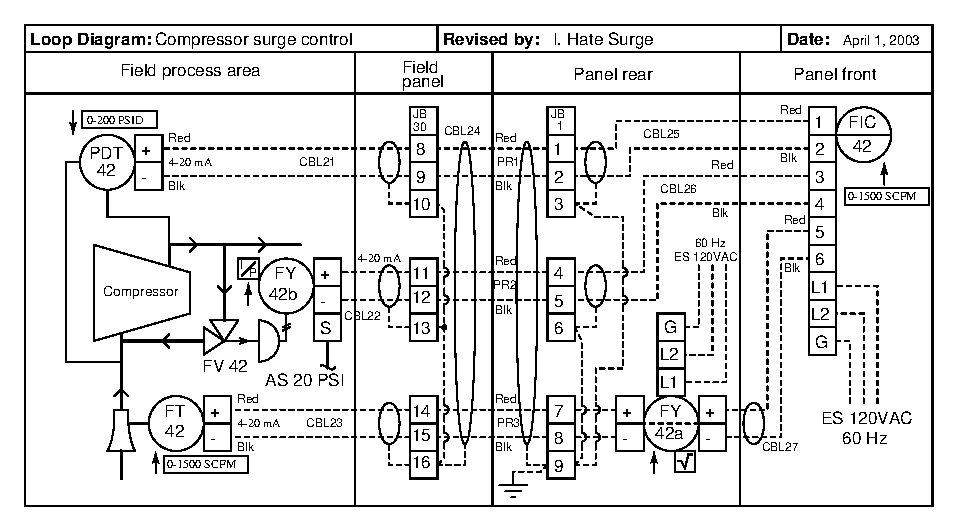
\includegraphics[width=15.5cm]{i00134x01.eps}$$

If the screw on terminal JB1-4 were to come loose, breaking the connection between the two wires joined at that point, what would this surge control valve do, and what effect do you think that would have on the compressor?

\vskip 20pt \vbox{\hrule \hbox{\strut \vrule{} {\bf Suggestions for Socratic discussion} \vrule} \hrule}

\begin{itemize}
\item{} Identify whether FV-42 is {\it fail-open} (FO) or {\it fail-closed} (FC).
\item{} What do the short arrows represent (located next to the individual instrument bubbles) in this loop diagram?
\end{itemize}

\underbar{file i00134}
%(END_QUESTION)





%(BEGIN_ANSWER)

If the screw on JB1-4 were to come loose, it would interrupt the current to the I/P transducer, thus making its pneumatic output fail low.  We know this because the upward-pointing arrow next to FY-42b denotes it as direct-acting (more mA = more air pressure out).  With low air pressure to the bypass valve, the valve will fail open (as indicated by the arrow on the valve stem symbol).  This will bypass flow from output to input on the compressor, reducing the amount of gas flow to the process.

\vskip 10pt

For your information, compressor surge is a fluid dynamic phenomenon whereby the blades in a non-positive-displacement compressor (e.g. axial or centrifugal vane) ``stall'' just like the wings of an airplane flying too slowly and/or at too great an angle of attack.  When the blades of a compressor stall, they lose ``traction'' on the compressed gas, unloading the mechanical driver (engine, motor, or turbine) and allowing the compressor to gain speed, then the blades will ``un-stall'' and re-load the driver, continuing the cycle.

The following passage is taken from Francis Shinskey's excellent book {\it Energy Conservation and Control}, published by Academic Press in 1978, describing compressor surge:

\vskip 10pt {\narrower \noindent \baselineskip5pt

``The most demanding aspect of controlling compressors is surge protection.  The problem lies in being unable to determine with absolute certainty the degree of approach to surge.  Once a compressor begins to surge, it will continue until corrective action is applied, so automatic protection is mandatory.  A small centrifugal compressor may surge several times without damage, but a 100,000-hp axial could require reblading after a single incident.''

\vskip 5pt

``When a compressor begins to surge, the suction flow falls to zero within a few milliseconds, reverses momentarily, and begins to recover in less than a half second.  If the situation is not corrected, the cycle repeats immediately, resulting in a series of thunderclaps less than a second apart.  The sudden fall in suction flow can be detected and used to open a recirculating valve, but not before at least one surge cycle is sustained.  To prevent surge from developing at all requires a control system which skirts the unstable area altogether.''

\par} \vskip 10pt

%(END_ANSWER)





%(BEGIN_NOTES)


%INDEX% Documentation, loop diagram: compressor surge control
%INDEX% Documentation, loop diagram: fault analysis

%(END_NOTES)


